\documentclass{ecmm427_assignment}
\usepackage{url} % required as the bibfile has a url in it
\usepackage{graphicx}
\graphicspath{ {./} }
\usepackage{float}

\bibliographystyle{abbrv}

\begin{document}

\title{Computer modelling and simulation\\ CW1 - Report}
\author{Kieran Bacon - 640041851}
\maketitle
\thispagestyle{empty}

\declaration
\newpage % forcing a new page to separate the body of the report from the coverpage

\tableofcontents
\thispagestyle{empty}

\newpage
\pagenumbering{arabic}

\section{Exercise 1}

\subsection{Python Solution}

For the M/M/C/C implementation, I have decided to construct it using the Python programming language. I have separated out the varies parts of the simulation into 4 classes: Event which represents the events caused by a client moving through the simulation; EventHandler which manages provides convenient methods to interact with the events; Servers which represents the enactment of work that is to be done within the system; and the Simulation itself, that makes use of these classes to produce a complete piece of software.

The simulation begins by generating an event list with a single arrival. This arrival event contains its own method of determining its time requirements within the simulation. The simulation then begins a while loop over the event list, extracting and processing each event until some evaluation criteria. Traditionally, the criteria would be the total time of the simulation or the number of arrivals. For this system, it has been encoded to terminate when a set number of arrivals occurs.

For an event that is of the type `arrival', the system begins by generating a new arrival event, providing the current simulation time as an argument. The simulation then checks to see if any servers are available. If none are free, the event is blocked and no further action is taken. Otherwise, the event is allocated a server and the type of the event is converted into a `departure'. The modified event is then placed back into the event handler for future evaluation.

For an event of type `departure', the server that was allocated to that event is freed and available to work on a new arrival. The departure event is then passed back to the event handler for storage.

\subsubsection{Event}
\begin{verbatim}
from numpy import log
import random

class Event:
    """ Class object to represent an event that occurs during the simulation """

    arrivalRate = 0.1     # Static arrival rate of all events
    departureRate = 0.01  # Static departure rate of all events

    def expon(mean_rate: float) -> float:
        """ Calculate a random value from a exponential distribution around a
        specified mean.

        Params:
            - mean_rate :: the mean of the exponential distribution.

        Returns:
            - float :: the randomly generated value for time.
        """
        return - (log(random.random())/mean_rate)

    def __init__(self, type: str, time: float):
        """ Initialise the event. Calculate the arrival time and departure time 
        of the event, from a given time instance.

        Params:
            - type :: Identification of state of event.(start/arrival/departure)
            - time :: A time setting, expected to be the simulation time at the 
                      point of creation.
        """

        # Record type
        self.type = type
        # Calculate the arrival time using an exponential distribution
        self.arrival_time = time + Event.expon(Event.arrivalRate)
        # Calculate the departure time using an exponential distribution 
        self.departure_time = self.arrival_time + Event.expon(Event.departureRate)

    def __str__(self) -> str:
        """ Protected function to allow str() to display an object 
        
        Returns:
            - str :: A string representation of the event.
        """
        return self.type + " event at time: " + str(self.time())

    def time(self) -> float:
        """ Returns the time of the event depending on its type.
        
        Returns:
            - float :: The time of the event depending on the type.
        """
        if self.type == "arrival":
            return self.arrival_time
        return self.departure_time

    def serviceTime(self) -> float:
        """ Return the service time of the event. 
        
        Returns:
            - float :: Difference in time between the arrival and departure of 
                       the event.
        """
        return self.departure_time - self.arrival_time

    def servedBy(self, serverID = None):
        """ Overloaded function to set the server that has been allocated to the
        event, or to return the server ID. As a server can only be allocated to 
        an event that must then depart, the event type is also changed.

        Params :
            - serverID :: The id that represents a server

        Returns:
            - None :: In the event that a server is being set, None is returned.
            - int  :: In the event that no parameter is given, the id of the
                      server of this event is given.
        """

        if serverID:
            self.type = "Departure"   # Change event type
            self.serverID = serverID  # Record server ID
            return

        return self.serverID
\end{verbatim}
\subsubsection{EventHandler}
\begin{verbatim}
from Event import Event, M1M2Event

class EventHandler:
    """ Event handler is tasked with managing a collection of events. The events
    that are to be enacted in the future are stored in order of execution
    separately from the blocked or departed events.
    """

    def __init__(self):
        """ Initialise the object variables """
        self.container = []  # Event list of future events
        self.departed = []   # Events that have been resolved
        self.blocked = []    # Arrivals that have been blocked from entry

    def add(self, event: Event) -> None:
        """ Add a new event into the handler correctly into the sorted event
        list.

        Params:
            - event :: Event to be stored in the list
        """

        # Look for index of correct insertation of event
        for i, e in enumerate(self.container):
            if e.time() > event.time():
                self.container.insert(i, event)
                return
        
        # No events in the list or event correctly placed at end of event list.
        self.container.append(event)
    
    def depart(self, event: Event) -> None:
        """ Store the departed event """
        self.departed.append(event)

    def block(self, event: Event) -> None:
        """ Store the blocked event """
        self.blocked.append(event)

    def next(self) -> Event:
        """ Remove the next event from the event list and return the event.

        Returns:
            - Event :: The next event to be enacted in the simulation
        """
        e = self.container[0]
        self.container = self.container[1:]
        return e
\end{verbatim}

\subsubsection{Servers}
\begin{verbatim}
class Servers:
    """ A collect of server ID, provides a collection of convenient functions to 
    interact with a server item. The servers are represented by an integer, 
    these server ids move back and forth from a free and busy list to keep
    track.
    """

    def __init__(self, num_servers: int):
        """ Initialise the server list. Server Ids fall in range 1 - the number
        of servers.
        
        Params:
            - num_servers :: The total number of servers in for the system.
        """
        self.free = list(range(1,num_servers+1))
        self.busy = []

    def __len__(self) -> int:
        """ Protected function allowing len() to determine the number of free
        servers.

        Returns:
            - int :: Number of free servers.abs
        """
        return len(self.free)

    def isFree(self) -> bool:
        """ Query if any servers are free.

        Returns:
            - bool :: True if server free, False if server not free.
        """
        return len(self) > 0

    def allocate(self) -> int:
        """ Remove next freely available server for allocation, record server is
        now busy.

        Returns:
            - int :: ServerID of the now allocated server.
        """
        server, self.free = self.free[0], self.free[1:]
        self.busy.append(server)
        return server

    def deallocate(self, server: int) -> None:
        """ Remove the server from the busy collection and ensure it is ready to
        be accessible for the next arrival event.

        Params:
            - server :: a serverID of a busy server
        """
        self.busy.remove(server)
        self.free.append(server)
\end{verbatim}
\subsubsection{Simulation}
\begin{verbatim}
from numpy import *

from EventHandler import EventHandler, M1M2EventHandler
from Servers import Servers
from Event import Event, M1M2Event

class MMCC:
    """ Simulation object tasked with conducting the MMCC system """

    def run(self, total_servers: int, total_arrival :int) -> None:
        """ Begin the simulation of a MMCC system. Process the information until
        termination criteria is meet.

        Params:
            - total_servers :: The number of servers that can handle clients at 
                               any one instance.
            - total_arrival :: The total number of clients that can be handled
                               within the simulation.
        """

        # Initialise the beginning parameters of the simulation
        self.servers = Servers(total_servers) # Set up server handler
        self.events = EventHandler()          # Set up the event handler

        startingEvent = Event("arrival", 0)   # Construct the first event object
        startingEvent.departure_time -= startingEvent.arrival_time # Reset times
        startingEvent.arrival_time = 0        # Reset times

        self.events.add(startingEvent)        # Create the first event

        # Begin iteration of events, record arrivals for checking
        self.num_arrival = 0
        while(self.num_arrival < total_arrival):

            # Collect next event from the event handler
            currentEvent = self.events.next()
            # Update simulation time
            self.sim_time = currentEvent.time()

            if currentEvent.type == "arrival":
                # Arrival event received
                self.num_arrival += 1 # Record number of arrivals

                # Create new arrival event
                self.events.add(Event("arrival", currentEvent.time()))

                # Check if any server is available
                if not self.servers.isFree():
                    self.events.block(currentEvent) # Arriving client is blocked
                    continue
                
                # Begin serving the client.
                currentEvent.servedBy(self.servers.allocate())

                # All event handler to manage departure
                self.events.add(currentEvent)

            else:
                # Departure event received
                self.servers.deallocate(currentEvent.servedBy()) # Free the server
                self.events.depart(currentEvent)                 # Record departure

    def blockingProbability(self) -> float:
        """ Calculate the blocking probability for the previous simulation run.
        
        Returns:
            - float :: Probability of blocking 
        """
        return len(self.events.blocked)/self.num_arrival
 
    def serverUtilisation(self) -> float:
        """ Calculate the server utilisation for the previous simulation run.
        
        Returns:
            - float :: Server utilisation value
        """
        return sum([e.serviceTime() for e in self.events.departed])/self.sim_time

    def report(self) -> None:
        """ Display the results of the simulation is a readible fashion. """
        
        print("\tEvents Handled ::") 
        print("\t\tArrival:", self.num_arrival)
        incomplete = self.num_arrival - (len(self.events.departed) + len(self.events.blocked))
        print("\t\tIncomplete events:", incomplete)
        print("\t\tDeparture:", len(self.events.departed))
        print("\t\tBlocked:", len(self.events.blocked))

        print("\tBlocking rate:", self.blockingProbability())
        print("\tServer Utilisation:", self.serverUtilisation()) 
\end{verbatim}
\subsubsection{MMCC script}

\begin{verbatim}
from Simulation import MMCC
from Event import Event
from pylab import *
from math import factorial

def blockingProbability(num_servers: int, arrival_rate: float, departure_rate: float) -> float:
    """ Static function to be able to analytical determine the expected blocking
    probability for a simulation of MMCC given its parameters.

    Params:
        - num_servers: The number of clients in the simulation
        - arrival_rate: The exponential mean of arrival for the clients
        - departure_rate: the exponential mean of the departure of the clients

    Return:
        - float: Blocking probability of the system
    """
    numerator = double(((arrival_rate/departure_rate)**num_servers)/double(factorial(num_servers)))
    demoninator = sum( [((arrival_rate/departure_rate)**k)/factorial(k) for k in range(1,num_servers)])
    return numerator/demoninator

def serverUtilisation(arrival_rate: float, departure_rate: float) -> float:
    """ Calculate the expected server Utilisation of the system with the given
    parameters.

    Params:
        - arrival_rate: The exponential mean of arrival for the clients
        - departure_rate: the exponential mean of the departure of the clients

    Returns:
        - float: Value representing the server utilisation value

    """
    return arrival_rate/departure_rate


if __name__ == "__main__":

    matplotlib.pyplot.show() # Allow plotting package to display figures
    machine = MMCC()         # Generate simulation machine

    # Initialise investigation parameters
    servers = 16                        # Number of servers in the simulation
    arrival_range = logspace(-2,-1,50)  # Range or arrival values to test
    departure_rate = 0.01               # Departure rate of simulation events
    clients = 10000                     # Number of client arrivals

    # Data structures to hold observations
    prob_blocking = [] # Probability of blocking evaluated from the simulation
    pred_blocking = [] # Predicted probability of blocking from an analytical model

    utilisation = []      # Recorded utilisation value from the simulation
    pred_utilisation = [] # Predicted utilisation value from an analytical model

    
    # Begin investigation
    index = 0 
    for i, arrival_rate in enumerate(arrival_range):
        Event.arrivalRate = arrival_rate # Set the arrival rate value

        # run the simulation 
        machine.run( total_servers = servers, total_arrival = clients )        

        # Collect the statistical information from the simulation
        probability = machine.blockingProbability()
        
        # Record simulation that yielded a blocking probability less than 0.01
        if probability < 0.01: index = i

        # Add information into data structures
        prob_blocking.append(probability)
        pred_blocking.append(blockingProbability(servers, arrival_rate, departure_rate))

        utilisation.append(machine.serverUtilisation())
        pred_utilisation.append(serverUtilisation(arrival_rate, departure_rate))

    # Display best simulation values
    print("Values for re-run on best arrival rate:")
    Event.arrivalRate = arrival_range[index]
    machine.run(total_servers = servers, total_arrival = clients)
    machine.report()
    print()

    # Statistical information about the progress of the investigation
    difference = [i-j for i, j in zip(prob_blocking, pred_blocking)]
    print("For blocking rate lower than 0.01:")
    print("\tArrival rate:", arrival_range[index])
    print("\tSimulation blocking probability:", prob_blocking[index])
    print("\tSimulations variance from predictions:", sum(difference)/len(difference) )

    # Plot the findings of the investigation for blocking probability
    figure()
    plot(arrival_range, prob_blocking, "b*", label="Simulation blocking percentage")
    plot(arrival_range, pred_blocking, "r--", label="Analytic blocking percentage")
    plot([0.01, arrival_range[index]], [prob_blocking[index]]*2, "y--", label="Setup with probability under 0.01")
    plot([arrival_range[index]]*2, [-0.0005, prob_blocking[index]], "y--")
    legend()
    ylabel("Blocking Probability")
    xlabel("Arrival rate")
    xlim(0.01, 0.1)
    ylim(-0.0005,0.025)
    show(block=True)

    # Plot the findings of the investigation for server utility
    figure()
    plot(arrival_range, utilisation, "b*", label="Utilisation of servers")
    plot(arrival_range, pred_utilisation, "r--", label="Predicted utilisation of servers")
    ylabel("Server Utility")
    xlabel("Arrival rate")
    legend()
    xlim(0.01, 0.1)
    show(block=True)
\end{verbatim}



\subsection{Investigation statistics}

\begin{figure}[H]
 \centering
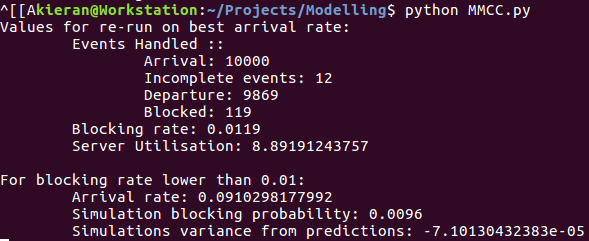
\includegraphics[scale=0.65]{MMCCOutput.png}
\caption{Terminal output generated when the MMCC script is run}
\end{figure}

\begin{figure}[H]
 \centering
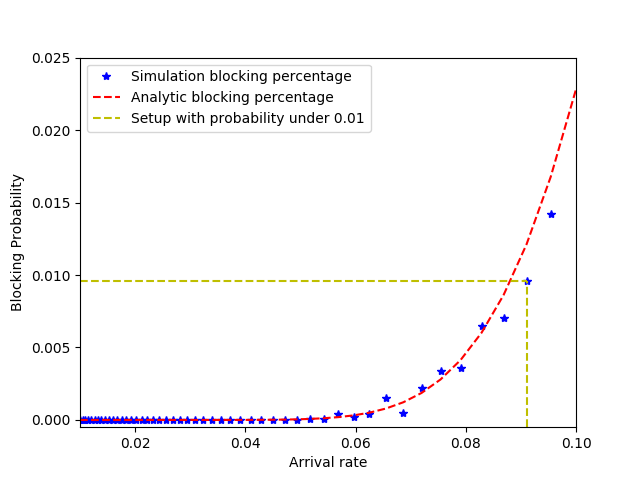
\includegraphics[scale=0.65]{MMCCBlockingProb.png}
\caption{A visualisation of the blocking probability compared with the analytical blocking probability. Also showing which solution was choosen and why.}
\end{figure}

\begin{figure}[H]
 \centering
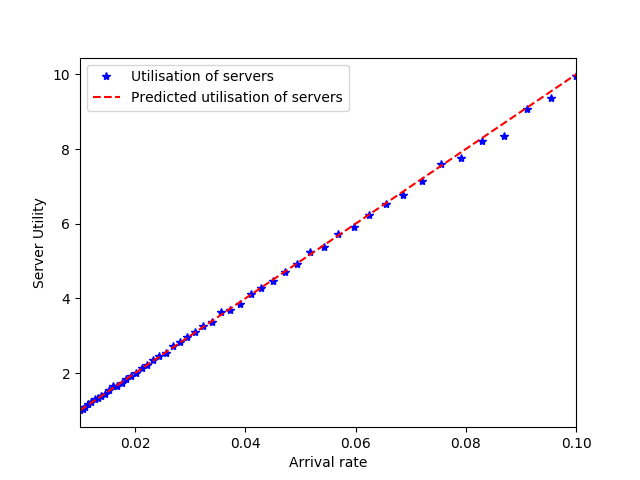
\includegraphics[scale=0.65]{MMCCUtilisation.png}
\caption{A visualisation that shows the server utility values against the expected values generated analytically.}
\end{figure}

Displaying the results against the expected values from the analytical models provides validity to the simulation. As their variance is extremely low there is an agreement between them upon the values I have given.

Figure 1 illustrates the input values for the simulation that achieved the greatest value for arrival rate with a probability beneath 0.01. That value was 0.0869... With an increase in the number of data points, I would expect the value would converge to a different optimum. The choice to do so would be depending on the stakeholder's requirement for precision.
 
\section{Exercise 2}

\subsection{Python Solution}

To implement M1+M2/M/C/C, I decided to you the python programming language. The core aspects of the simulation follow closely to the M/M/C/C simulation. Primarily the difference is in the manner the events pass through the simulation.

Events have been adapted to contain information about the arrival path that have originated from. This information is used to determine the arrival and departure time of the event, but to also understand what kind of arrival event needs to be generated by the simulation class when it is collected from the event list.

The event list is altered to be more considerate of the two streams of arrivals by separating the blocked elements. Additionally a start function is also added to generate the first two events for both streams in an unbiased manner, additiona the function is tasked with ensuring that statistical information isn't skewed by the warm up period of the events.

The simulation is changed to give priority to the handover calls. Instead of simply checking a free server, the program is altered to check two possible conditions of the state of the servers in a lazy optimisation format.

Included below are extended classes that were used in place of the M/M/C/C classes to come to a result, along with the script used.

\subsubsection{Updated Event}
\begin{verbatim}
class M1M2Event(Event):
    """ Event object responsible for recording the time for the event and the 
    type of event. The path on which the event affects the mean of the times
    exponential distribution.
    """
    # Static arrival rates for the hand over and new call paths
    priorities = {"handover":0.1, "newcall": 0.1}  
    departureRate = 0.01   # Static departure rates for events

    def __init__(self,path, type, time):
        """ Initialise the values for the event """
        self.path = path
        self.type = type
        self.arrival_time = time + Event.expon(M1M2Event.priorities[path])
        self.departure_time = self.arrival_time + Event.expon(M1M2Event.departureRate)
\end{verbatim}
\subsubsection{Updated EventHandler}
\begin{verbatim}
class M1M2EventHandler(EventHandler):
    """ Adaptation of the event handler object to have separate collections for
    the hand over rate, new call rate blocked events. Additionally functionality
    to ensure non bias creation of the initial arrival events is introduced
    """

    def __init__(self):
        """ Initialising the data structures for the object """
        self.container = [] # Event list of future events
        self.departed = []  # Events that have departed from the simulation
        self.hblocked = []  # Hand over events that were blocked
        self.nblocked = []  # New call events that were blocked

    def start(self) -> None:
        """ Generate both event types and introduce them into the event list,
        ensuring the no warm up period is included to prevent statistical skew.
        """

        # Create both event types objects
        arrivals = [M1M2Event("handover", "arrival", 0), M1M2Event("newcall", "arrival", 0)]

        # Identify which of the two occur first
        startTime = min([arrivals[0].time(), arrivals[1].time()])

        for e in arrivals:
            # Remove the warm up time from event times
            e.arrival_time = e.arrival_time - startTime
            e.depature_time = e.departure_time - startTime

            # Store the events
            self.add(e)

    def block(self, event: M1M2Event) -> None:
        """ Overwriting Event block function, to include functionality of two 
        different blocked collections

        Params:
            - event: Event to be blocked
        """
        if event.path == "handover":
            self.hblocked.append(event)
        else:
            self.nblocked.append(event)
\end{verbatim}
\subsubsection{Updated Simulation}
\begin{verbatim}
class M1M2CC(MMCC):

    def run(self, total_servers: int, total_arrival :int, threshold: int) -> None:
        """ Begin the simulation and record the system variables during execution.

        Params:
            - total_servers :: The number of servers that can handle clients at 
                               any one instance.
            - total_arrival :: The total number of clients that can be handled 
                               within the simulation.
            - threshold :: The number of servers that must remain open for top 
                           priority callers.
        """

        # Initialise the beginning parameters of the simulation
        self.servers = Servers(total_servers) # Set up server handler
        self.events = M1M2EventHandler()      # Set up the event handler
        self.events.start()                   # Create the first event

        # Begin iteration of events, record arrivals for checking
        self.num_arrival = 0
        self.arrival = {"handover": 0, "newcall": 0}
        while(sum(self.num_arrival) < total_arrival):

            # Collect next event from the event handler
            currentEvent = self.events.next()
            # Update simulation time
            self.sim_time = currentEvent.time()

            if currentEvent.type == "arrival":
                # Arrival event received
                priority = currentEvent.path
                self.num_arrival += 1
                self.arrival[priority] += 1

                # Create new arrival event
                self.events.add(M1M2Event(priority, "arrival", currentEvent.time()))

                # Check server availablity
                if (len(self.servers) > threshold) or \
                   (priority == "handover" and self.servers.isFree()) :
                    
                    # Begin serving the client.
                    currentEvent.servedBy(self.servers.allocate())

                    # All event handler to manage departure
                    self.events.add(currentEvent)
                    continue
                
                # No servers were available therefore the event is blocked
                self.events.block(currentEvent) # Arriving client has been blocked

            else:
                # Departure event received
                self.servers.deallocate(currentEvent.servedBy()) # Free the server
                self.events.depart(currentEvent)                 # Event recorded as departed.

    def blockingProbability(self):
        """ Calculate the blocking probability for the previous simulation run.
        
        Returns:
            - float :: Probability of blocking 
        """

        HFP = len(self.events.hblocked)/self.arrival["handover"] \
              if self.arrival["handover"] else 0
        CBP = len(self.events.nblocked)/self.arrival["newcall"] \
              if self.arrival["newcall"] else 0
        return CBP + (10 * HFP)

    def report(self) -> None:
        """ Display the results of the simulation is a readible fashion. """
        
        print("\tEvents Handled ::") 
        print("\t\tArrival:", self.num_arrival)
        print("\t\tHandover:", self.arrival["handover"])
        print("\t\tNew call:", self.arrival["newcall"])
        incomplete = self.num_arrival - \
            (len(self.events.departed) + len(self.events.hblocked) + len(self.events.nblocked))
        print("\t\tIncomplete events:", incomplete)
        print("\t\tDeparture:", len(self.events.departed))
        print("\t\tBlocked:", len(self.events.hblocked) + len(self.events.nblocked))
        print("\t\tHandover blocked:", len(self.events.hblocked))
        print("\t\tNew call blocked:", len(self.events.nblocked))

        print("\tBlocking rate:", self.blockingProbability())
        print("\tServer Utilisation:", self.serverUtilisation())  
\end{verbatim}
\subsubsection{M1+M2/M/C/C script}
\begin{verbatim}
from Simulation import M1M2CC
from Event import M1M2Event as Event
from pylab import *
from math import factorial

def blockingProbability(num_clients: int, threshold: int, ho_rate: float, \
                        c_rate: float, d_rate: float) -> float:
    """ Blocking probability function for a m1/m2/m/c/c type simulation, it 
    gives consideration to both paths of arrival and the priority aspects of
    each path. This function unfortunately did not provide reasonable results 
    for the validity checking but I have left is in as a work in progress.

    Params:
        - num_clients: The number of arrivals the system is to experience from 
                       both paths.
        - threshold: The number of reserved servers in the system for the hand 
                     over path.
        - ho_rate: The hand over arrival rate.
        - c_rate: The new call arrival rate.
        - d_rate: The departure rate for a given arrival.

    Returns:
        - float: Blocking probability of the simulation set up.
    """

    diff = num_clients - threshold

    a = sum([ (factorial(k)**-1)*(((ho_rate+c_rate)/d_rate)**k) for k in range(diff)])
    b = 0
    for k in range(diff + 1, num_clients):
        x = (((num_clients-factorial(threshold))*factorial(k-(diff)))**-1)
        y = (((ho_rate+c_rate)/d_rate)**(diff))
        z = ((ho_rate/d_rate)**(k-num_clients+threshold))
        b += x*y*z

    p0 = a + b

    a = ((num_clients-factorial(threshold))*factorial(threshold))**-1
    b = ((ho_rate + c_rate)/d_rate)**(diff)
    c = (ho_rate/d_rate)**num_clients

    return a*b*c*(p0**-1)


if __name__ == "__main__":

    matplotlib.pyplot.show() # Prepare python for plotting
    machine = M1M2CC()       # Construct a simulation object
    
    # Initialise investigation parameters
    handover_range = logspace(-6, -1, 50) # Range of hand over arrival rate
    Event.priorities["newcall"] = 0.1             # Set new call arrival rate
    Event.departure_rate = 0.01

    prob_blocking = []

    for p in handover_range:
        Event.priorities["handover"] = p
        machine.run(16,10000,2)
        prob_blocking.append(machine.blockingProbability())

    figure()
    plot(handover_range, prob_blocking, "b*", label="ABP blocking percentage")
    plot([handover_range[0], handover_range[-1]], [0.02]*2, \
        'r--', label="Target probability of 0.02")
    ylabel("ABP blocking probability")
    xlabel("Handover arrival rate")
    legend()
    xlim(handover_range[0], handover_range[-1])
    xscale("log")
    show(block=True)

    call_range = linspace(0.01, 0.08, 50)
    Event.priorities["handover"] = 0.03
    Event.departure_rate = 0.01

    prob_blocking = []
    index, best_prob = 0 , 0

    for i, c in enumerate(call_range):
        Event.priorities["newcall"] = c
        machine.run(16,10000,2)
        prob = machine.blockingProbability()
        if prob < 0.02: index, best_prob = i, prob
        prob_blocking.append(prob)
    

    print("Report from rerun on best proposed call arrival rate:")
    Event.priorities["newcall"] = call_range[index]
    machine.run(16,10000,2)
    machine.report()
    print("")
    
    print("For Aggregated blocking rate below 0.02:")
    print("\tCall arrival value:", call_range[index])
    print("\tBlocking value:", best_prob)

    figure()
    plot(call_range, prob_blocking, "b*", label="ABP blocking percentage")
    plot([0.01, call_range[index]], [prob_blocking[index]]*2, "r--", \
        label="Setup with probability under 0.02")
    plot([call_range[index]]*2, [-0.0005, prob_blocking[index]], "r--")
    ylabel("ABP blocking probability")
    xlabel("New call arrival rate")
    xlim(0.01,0.08)
    ylim(-0.005, 0.2)
    legend()
    show(block=True)
\end{verbatim}

\subsection{Investigation into aggregated blocking probability}

\begin{figure}[H]
 \centering
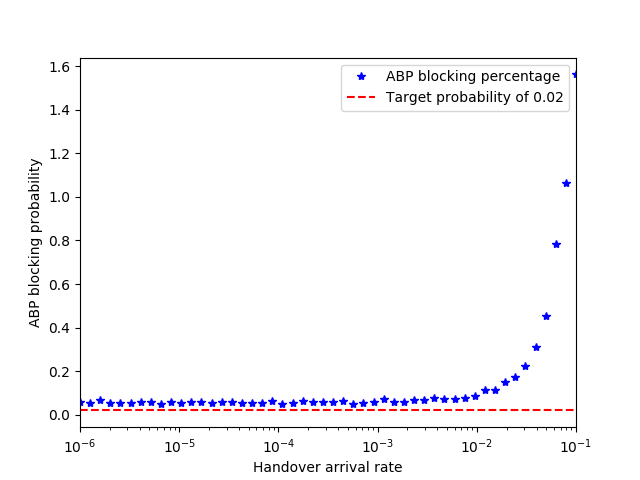
\includegraphics[scale=0.65]{M1+M2MCCInvestigation.png}
\caption{A visualisation of changing handover rate when attempting to reduce ABP under 0.02}
\end{figure}

We can see in figure 4 that regardless of the value set for the arrival rate of the `hand over' process, the value is always above the target. This is due to the fact that blocking will occur naturally within the second arrival path with a probability greater than 0.02. As the value of the rate of the hand over tends to zero, the aggregated blocking probability tends to this value. The overall system becomes similar to an M/M/C/C simulation with the number of servers equal to the server number minus the reserved server number e.g. $c-n$.

\begin{figure}[H]
 \centering
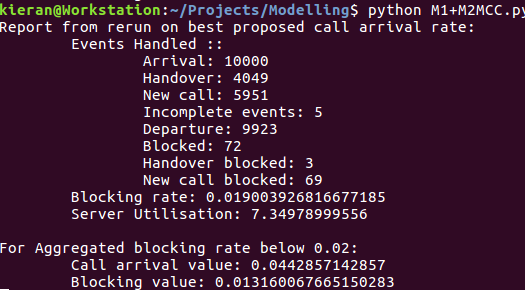
\includegraphics[scale=0.65]{M1+M2MCCOutput.png}
\caption{Terminal output generated when the M1+M2/M/C/C script is run.}
\end{figure}

\begin{figure}[H]
 \centering
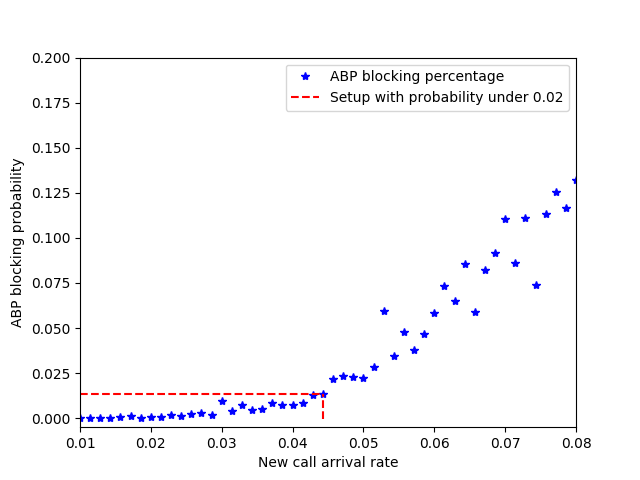
\includegraphics[scale=0.65]{M1+M2MCCABP.png}
\caption{A visualisation that shows the ABP values against arrival rate of the new call path.}
\end{figure}

\end{document}
